\documentclass[11pt,a4paper]{article}
\usepackage[czech]{babel}
\usepackage[utf8]{inputenc}
\usepackage{times}
\usepackage{url}
\usepackage[textwidth=15.2cm,textheight=23cm]{geometry}
\usepackage{xcolor}

\usepackage{graphicx}

%\usepackage{fancyvrb}
%\DefineVerbatimEnvironment{verbatim}{Verbatim}{}

\usepackage[bf]{caption}

\usepackage[hyperindex,
  plainpages=false,
  pdftex,
  colorlinks,
  pdfborder={0 0 0},
  pdfpagelabels]{hyperref}

\pdfcompresslevel=9

\newcommand{\myincludegraphics}[4]{
  \begin{figure}[!h]
  \centering
  \includegraphics[#1]{#2}
  \caption{#3.} \label{#4}
  \end{figure}
}

% titulní stránka a obsah
\newcommand{\titlepageandcontents}{
  \begin{titlepage}

\vspace*{1cm}

\begin{figure}[h]
  \centering
  
\includegraphics[height=6cm]{images/fit.pdf}
\end{figure}

\vspace*{20mm}

\begin{center}
\begin{huge}
Vysoké učení technické v Brně\\
Fakulta informačních technologií
\end{huge}
\end{center}

\vspace*{20mm}

\begin{center}
\begin{Huge}
\subject{} \\
\end{Huge}
\begin{huge}
Státnicové okruhy MSZ 2015\\
\end{huge}
\end{center}


\end{titlepage}


  \pagestyle{plain}
  \pagenumbering{roman}
  \setcounter{page}{1}
  %\tableofcontents

  \newpage
  \pagestyle{plain}
  \pagenumbering{arabic}
  \setcounter{page}{1}
}

\def\uv#1{\iflanguage{english}{``#1''}%
                              {\quotedblbase #1\textquotedblleft}}%

\newcommand\todo[1]{\textcolor{red}{[[TODO: #1]]}}
\newcommand\blindtextGray{\textcolor{gray}{\blindtext}}
\newcommand\comment[1]{}

\newcommand\subject[1]{Předmět}


% vim:set ft=tex expandtab enc=utf8:

\usepackage{amsmath}
\usepackage{moreverb}
\usepackage{float}


\renewcommand\subject[1]{PDS}

\begin{document} \sloppy
\titlepageandcontents

\section{Sítě Peer-to-Peer (P2P), Milgramův problém malého světa, model sítě P2P, směrování v P2P
sítích, strukturované a nestruktorvané sítě}
\subsection{Milgramův problém malého světa}
\begin{itemize}
\item Základ pro P2P sítě.
\item Potřebuji předat informaci člověku, kterého znám (mám informace o tom, kde se narodil atp.), ale neznám jeho adresu. Jsem shopen mu zásilku předat, aniž bych ji posílal klasickou poštou, jenom skrze lidi, které on zná a já znám (známé mých znamých)? 
\item Tato otázka vychází z poznatku jaká je pravděpodobnost, že se znají dva náhodně vybraní lidé. A pokud se neznají osobně, tak přes kolik známých se znají.
\item V podstatě hledáme matematické struktury ve společnosti. Máme stovky tisíc bodů a ptáme se přes kolik mezilehlých bodů je možné vytvořit nejkratší cestu pro dva libovlné uzly.
\item Závěr zní, že jedinci, kteří používají \textbf{pouze lokální informace}, jsou \textbf{velmi efektivní} ve vytvoření nejkratší cesty mezi dvěma body v sociální síti. Z toho plyne, že propojení mezi dvěma jedinci v síti je možné pomocí malé posloupnosti známých.
\item Otázkou je, zda existuje decentralizovaný aloritmus, který najde řetězec mezi dvěma libovolnými body. Odpoveď je \textbf{ano, existuje}.
\end{itemize}
\subsubsection{Milgramův experiment}
\begin{itemize}
\item Úkolem bylo doručit dopis příteli v jiném státě.
\item Jako odesilatele vybral náhodných 160 lidí (předpoklad byl, že odesilateli byly zděleny informace o adresátovi -- jaké má povolání, kde studovat atp.).
\item Dopis bylo možné předávat jenom skrze známé.
\item Každý, kdo dostal zásilku, posílal potrzující dopis zpátky na Hradvard (výchozí bod).
\item Výsledkem bylo, že nejkratší řetěz zpráv vedl přes 2 lidi, nejdelší přes 11 a medián bylo 5 lidí. Závěr tedy je, že stačí 5 lidí.
\end{itemize}

\subsection{Peer--to--Peer sítě}
%---obrazek
\begin{figure}[h!]
\begin{center}
\scalebox{0.8}{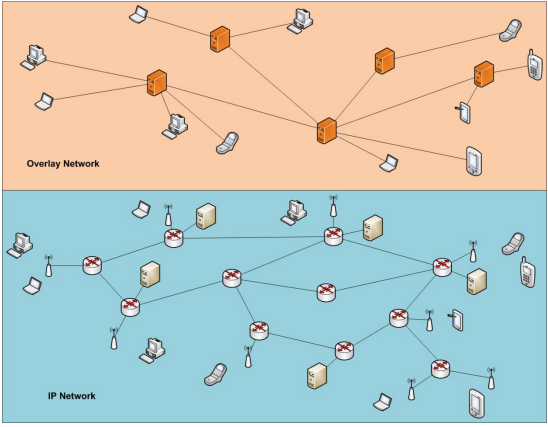
\includegraphics{images/overlay.png}}
\caption{Overlay u P2P sítí (oranžové).}
\label{p2p_overlay}
\end{center}
\end{figure}
%---konec obrazek
\begin{itemize}
\item P2P sítě jsou postavené nad IP, ale mají:
\begin{itemize}
\item Jinou koncepci architektury -- odlišná role uzlů.
\item Jiný způsob adresování -- adresování obsahem.
\item Jiný přístup ke směrování -- uzly se odpojují/připojují libovolně.
\item Jiné vlastnosti sítí -- samo--organizace, decentralismus.
\end{itemize}
\item Zdroje jsou dostupné všem -- slouží především pro sdílení zdrojů.
\item Základní operace v P2P sítích: připojení uzlu, odpojení uzlu a vyhledání objektu.
\item Všichni účastníci něco do sítě přinášejí a něco si z ní odnášejí (sdílím a stahuji).
\item Základem sítí P2P je \textbf{overlay} (vlastní nezávislá síť -- viz obrázek \ref{p2p_overlay}) -- síť, která je vybudovaná nad fyzickou architekturou (uzly z overlay se mapují na fyzické). Mezi uzly existuje komunikace a protokol -- řešeno speciálním SW.
\item Směrování u všech druhů P2P sítí je na základě pouze \textbf{lokální} informace.
\end{itemize}
\subsubsection{Struktura logické sítě overlay}
\begin{itemize}
\item Jedná se o orientovaný graf.
\item Operace připojení/odpojení uzlů.
\item Množina sousedů uzlu $p$ je dána \textbf{relací sousedství (neighborhood)} -- souvisí s vyhledáváním a říká, že pro každý uzel $p$ můžu mít množinu sousedních uzlů $N(p)$.
\item Důležitý parametr je \textbf{poloměr grafu} -- maximální vzdálenost mezi dvěma uzly grafu (menší poloměr -- rychlejší vyhledávání).
\end{itemize}
\subsubsection{Typy P2P sítí}
\begin{itemize}
\item \textbf{Pravé P2P sítě} -- všechny uzly mají stejný význam (tj. pokud odeberu uzel ze sítě nemá to to vliv na ztrátu schopnosti sítě poskytovat dané služby).
\item \textbf{Hybridní P2P sítě} -- několik typů uzlů. Potřeba centrálního uzlu pro poskytování části nabízených služeb (tento bod slouží k autentizaci, indexování atp.). Jedná se o kombinaci P2P a klient--server.
\end{itemize}
\subsubsection{Model P2P sítě}
%---obrazek
\begin{figure}[ht!]
\begin{center}
\scalebox{0.8}{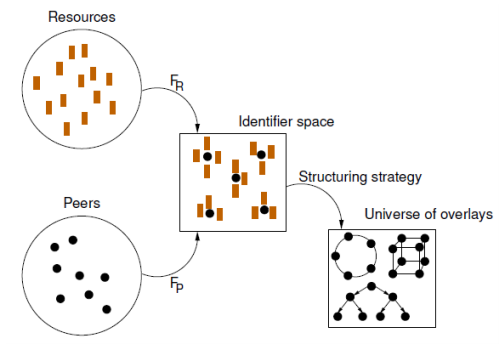
\includegraphics{images/model_p2p.png}}
\caption{Model P2P sítí.}
\label{p2p_model}
\end{center}
\end{figure}
%---konec obrazek
Model P2P sítě (viz obrázek \ref{p2p_model}) se skládá z komponent:
\begin{itemize}
\item Jmenný prostor $I$ -- prostor jmen, identifikuje uzly (dle hashe nějaké charakteristiky -- např. hash z IP, hash privátního klíče atp.) a zdroje (dle hashe názvu souboru, hashe názvu článku$\ldots$), které jsou tam připojené. \textbf{Musí obsahovat metriku blízkosti} (definice metriky viz MAT) kvůli vyhledávání atp.
\item Množina uzlů (peers) $P$
\item Množina zdrojů (resources) $R$ -- soubory, články$\ldots$
\item Mapování objektů $F_R : R \rightarrow I$ -- Přidělí zdrojům identifikátor z I.
\item Mapování uzlů $F_P : P \rightarrow I$ -- Přidělí uzlům jednoznačný identifikátor.
\item Struktura logické sítě -- vytváří vlastní síť z identifikačního prostoru.
\end{itemize}

\end{document}

